In this chapter, we introduce Machine Learning and Blockchain concepts and definitions that are regarded as necessary prior knowledge for understanding the remaining chapters of this report.

\section{Machine Learning}\label{fundamentals:machine_learning}

Machine Learning is a sub-field of Artificial Intelligence that builds models based on statistical and algorithmic concepts in order to detect relevant patterns based on prior experience \cite{geron_2019}. This models learn and adapt without explicit instructions when given new data during a process called training. The data is usually structured as vectors in a multi-dimensional space, such that each vector is an \textit{instance} and each dimension is a \textit{feature}.

There are three main categories of ML algorithms: \textit{supervised learning}, \textit{unsupervised learning} and \textit{reinforcement learning} \cite{geron_2019}. Each category performs different types of tasks on different types of data. This study focuses only on classification problems in supervised learning settings.

In supervised learning, algorithms build mathematical models using a set of input samples, which are vectors from a feature space, and expected outputs for each sample. This type of data is known as labeled data, as there is a label for each sample. During training, algorithms provide the model with the input samples and improve the model by comparing its output with the expected outputs. Supervised learning problems can be divided into \textit{regression problems}, if the output is a continuous variable, or \textit{classification problems}, if the output is a discreet variable.

% \subsubsection{Unsupervised Learning}

% In unsupervised learning, in contrast to supervised learning, algorithms build mathematical models using unlabeled data. Therefore, there are no expected outputs that can be directly compared to the model's output. Some common problems solved by unsupervised learning are \textit{clustering}, \textit{dimensionality reduction} and \textit{anomaly detection}.

% \subsubsection{Reinforcement Learning}

% In reinforcement learning, models must learn the best action to take according to the current environment, receiving either \textit{rewards} or \textit{penalties} if they perform a good, or bad action, respectively.

\section{Federated Learning}\label{fundamentals:federated_learning}

Federated Learning is a ML technique where different clients collaboratively train a model under the supervision of a centralized orchestrator. Clients are distributed heterogeneous devices with their own computing resources and they are responsible for producing and maintaining their own data \cite{9084352}. The data is assumed to be non independent or non identically distributed (\textit{non-iid}).

Since clients are heterogeneous and distributed, different communication costs and response times are normal. In addition, some clients may operate under constrained networks with either low or limited bandwidth. Therefore, it is important that new FL techniques ensure that communication and resource usage is minimized.

During the training process, the raw data never leaves the clients and only a representation of the model, such as model weights, is exchanged with the server in order to compute the global model. However, model weights can be target of inference attacks and leak secret information \cite{10.1145/3298981}.  Consequently, new innovations must be compatible with techniques that guarantee privacy, such as differential privacy, homomorphic encryption, secure multiparty computation or other cryptographic protocols.

After each round of training, the central orchestrator aggregates the local updates. Usually, this is done using a formula known as Federated Averaging (\textit{FedAvg}) \cite{10.48550/arxiv.1602.05629}, which calculates the weighted average of all clients $k \in K$ weights $w^k$:

\begin{equation}
w_{t+1} = \sum_{k \in K} \frac{n_k}{n} w_{t+1}^k
\end{equation} \label{eq:fedavg}

Where $n_k$ is the number of samples that the client $k$ used to train and $w_{t+1}^k$ the weights of client $k$ at round $t+1$.

\subsection{Architectures of Federated Learning}

Federated Learning can be broadly divided into three main architectures \cite{10.1145/3298981, 10.1145/3412357} that regard, for the most part, to the different data partition among the clients: Horizontal Federated Learning, Vertical Federated Learning and Federated Transfer Learning. This study focuses on Horizontal and Vertical Federated Learning.

\begin{figure}[!ht]
    \centering
    \centering
    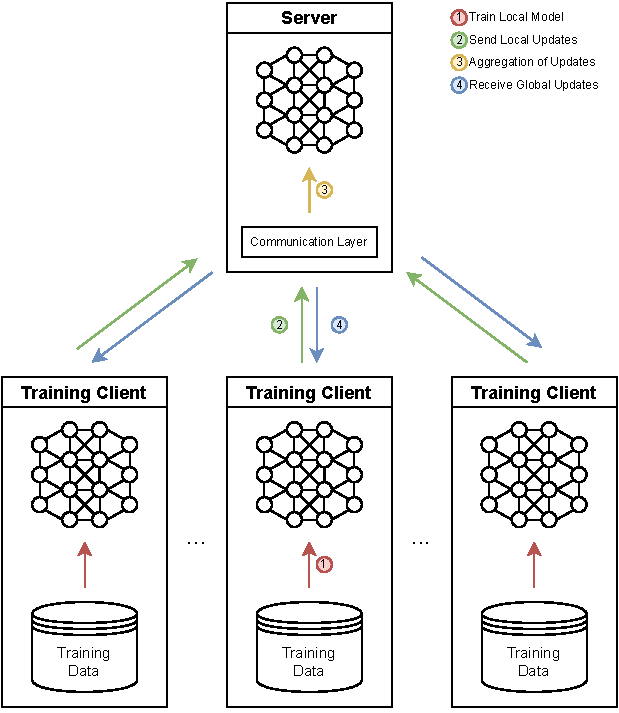
\includegraphics[width=0.6\textwidth]{graphics/hfl-architecture.pdf}
    \caption{Horizontal Federated Learning Architecture}
    \label{fig:hfl_arch}
\end{figure}

In \textit{Horizontal Federated Learning} (HFL), clients with the same data structure collaborate to build a single model. In other words, the different data sets in the different clients share the same feature space, but not the sample space. For example, two banks have similar businesses (feature space), but target different clients (sample space). The architecture of HFL, depicted in \autoref{fig:hfl_arch}, consists of multiple clients training a model, while the central server performs the aggregation of all local updates.

In \textit{Vertical Federated Learning} (VFL), clients share an intersecting sample space, but different feature spaces. For example, two companies operating in the same city have a similar client base (sample space), but different areas of operation (feature space). The architecture of VFL, depicted in \autoref{fig:vfl_arch}, is similar to the one of HFL. However, it includes an additional step to calculate the Private Set Intersection (PSI) since the clients do not share the exact same sample space.

\begin{figure}[t] % !ht
    \centering
    \centering
    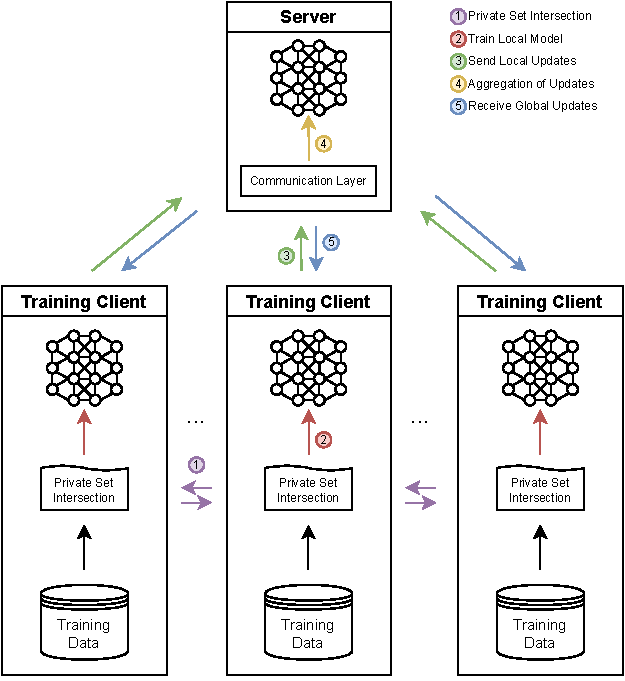
\includegraphics[width=0.6\textwidth]{graphics/vfl-architecture.pdf}
    \caption{Vertical Federated Learning Architecture}
    \label{fig:vfl_arch}
\end{figure}

% \subsubsection{Federated Transfer Learning}

% In Federated Transfer Learning (FTL), clients do not share a sample space, nor a feature space. This technique is similar to regular transfer learning, where a model is previously trained on a data set and then applied to a new similar, but different, data set. For example, two different companies that operate in different countries across the world have a different feature and sample space. However, it may be useful to transfer knowledge between different domains.

\section{Blockchain}\label{fundamentals:blockchain}

A blockchain is an immutable distributed ledger of transactions maintained by several computers, also known as nodes, linked through a peer-to-peer network. The concept of blockchain was first introduced by Stuart Haber and W. Scott Stornetta in 1991 \cite{10.48550/ARXIV.1810.06130}, being popularized by Satoshi Nakamoto in 2008 with the introduction of the cryptocurrency Bitcoin \cite{nakamoto2009bitcoin}.

\begin{figure}[h]
    \centering
    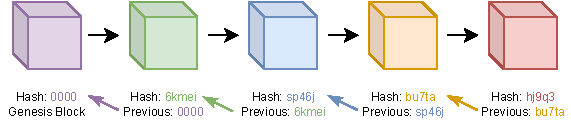
\includegraphics[width=0.8\textwidth]{graphics/blockchain.pdf}
    \caption{Blockchain Representation}
    \label{fig:blockchain_blocks}
\end{figure}

In a blockchain, the data is structured as blocks, as can be seen in \autoref{fig:blockchain_blocks}. Each block contains a certain amount of transactions and links to the previous block via a cryptographic hash, forming a chain. Hence, blockchain. This guarantees fidelity and trust without requiring a trusted third party, which is why it is called a \textit{trustless} system. In addition, since the record is immutable and decentralized, all transactions can be transparently viewed by others.

As mentioned beforehand, a blockchain is maintained by several nodes in a peer-to-peer network. As transactions come in, nodes compete in order to generate the next block. Since it is a decentralized process, multiple nodes will try to create the next block of the chain in parallel. In order to reach an agreement between the nodes, a consensus algorithm is used. The consensus algorithm allows to reach an agreement between multiple decentralized nodes without requiring a singular node to be in charge.

\begin{figure}[h]
    \centering
    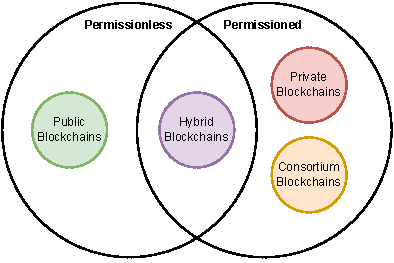
\includegraphics[width=0.5\textwidth]{graphics/blockchain-types.pdf}
    \caption{Blockchain Types}
    \label{fig:blockchain_types}
\end{figure}

There are four different types of blockchain: public, private, consortium and hybrid. Some of these are permissionless, which means that anyone can join the network, while some are permissioned, which means that only allowed parties can join the network. This separation can be visualized in \autoref{fig:blockchain_types}. They work as follows:

\begin{itemize}
    \item \textit{Public Blockchains}. They sit on the permissionless end of the spectrum and therefore anyone can join and participate in the network. There is no central authority.

    \item \textit{Private Blockchains}. In opposition to public blockchains, private blockchains sit on the opposite side of the spectrum, being a permissioned blockchain with a single central authority. This blockchains can only be accessed by allowed parties and they are usually used within organizations.

    \item \textit{Consortium Blockchains}. Similarly to private blockchains, consortium blockchains are also permissioned. However, instead of being controlled by a single authority, they are controlled by a group of different authorities.

    \item \textit{Hybrid Blockchains}. The hybrid blockchains have features of both permisionned and permissionless blockchain systems. On one hand, they are usually controlled by a single authority. On the other hand, they have a mixed usage of permissioned and permissionless protocols running in parallel for different use cases.
\end{itemize}

\subsection{Smart Contracts}

Some blockchain platforms, such as Ethereum \cite{wood2014ethereum}, provide functionality for smart contracts. Smart contracts are small computer programs that live within the blockchain and automatically run when predetermined conditions are met. As they live in the blockchain, they are trustless and are typically used to automate the execution of agreements. This way, every party involved in the agreement is certain that it will be honored once the conditions of the agreement are met.

\section{Blockchain-based Federated Learning}\label{fundamentals:blockchain}

\todo{Explain why BFL exists and what it attemps to solve and show an architecture of such system., MENTION REWARDS}